\setcounter{page}{1}
Para além da pesquisa acadêmica, a Computação em Nuvem, hoje se faz presente na vida de pessoas e empresas, integrando-se em suas rotinas e atividades do cotidiano e estabelecendo-se como uma importante e fundamental meio computacional. 

O conceito tem se tornando um paradigma cada vez mais reconhecido e utilizado. Inúmeras empresas tem apoiado e incentivado o uso e o seu desenvolvimento, assim como o meio científico. Atualmente, os exemplos desse paradigma de computação oferecem diversas opções para armazenamento ou processamento de dados, tais como, a \textit{\sigla{S3}{Simple Storage Service}} da Amazon, Bigtable do Google, ou PNUTS do Yahoo \cite{Binnig2009}. \citeonline{vazquez2014} exemplificam com o crescimento do Instagram, que construiu a sua base de usuários de mais de 150 milhões de usuários em menos de quatro anos usando soluções em nuvem.

O aumento da popularidade da computação em nuvem é impulsionado pelas vantagens oferecidas e pelo modelo dinamicamente escalável e o rápido desenvolvimento nos últimos anos levou a uma grande quantidade de publicações. O interesse no meio acadêmico e da indústria têm levado a uma quantidade considerável de publicações de artigos científicos nos últimos anos \cite{Heilig2014}. Como apresentado nos trabalhos de \citeonline{Heilig2014} e \citeonline{Yang2012}, o número de pesquisas têm concentrado esforços na resolução de problemas que em geral envolvem desempenho e/ou garantia de requisitos de Qualidade de serviço (\textit{\sigla{QoS}{Quality of service}}). 

Nessa área existe uma grande preocupação por parte dos provedores de computação em garantir QoS de uma forma eficiente. Em termos de recursos, significa que os recursos virtuais (\textit{\sigla{VMs}{Virtual Machines}}) e/ou físicos tem devem ser alocados de forma autônoma, para que possam responder às influências externas, como a carga de trabalho. Observa-se, por outro lado que, os \textit{data center} são muitas vezes subutilizados devido ao excesso de provisionamento, bem como as demandas de recursos que variam no tempo de acordo com os sistemas \cite{Padala2007}. \citeonline{Inomata2011} afirmam que tempo e dinheiro são investido para projetar, construir, configurar, monitorar e manter recursos computacionais e que o futuro da computação em nuvem é o auto gerenciamento e a atribuição de recursos automáticos aos seus consumidores com base na carga de trabalho.

Atualmente, com o advento e crescimento das aplicações intensivas de dados, que lidam com grandes volumes em tempo real, a dinâmica do sistema passa ser apreciável, fenômeno frequentemente não perceptível claramente para os sistemas computacionais. Na prática, tais aplicações, de grande volume de dados, tendem a operarem com cargas de trabalho variante no tempo, causando inúmeras dificuldades. A computação em nuvem oferece uma infraestrutura elástica ou escalável que pode ser utilizada para obter recursos sobdemanda; no entanto, um problema em aberto é decidir sobre a correta alocação de recursos ao implantar a nuvem \cite{Cervino2012}. De modo geral, um sistema dinâmico não apresenta os efeitos das ações da carga de forma imediata. Por exemplo, a velocidade de um carro não muda imediatamente quando o pedal do acelerador é acionado assim como a  temperatura em uma sala muda instantaneamente quando um aquecedor é ligado.

Este comportamento dinâmico começa a ser apreciado em grande sistemas computacionais, quanto um súbito aumento de requisições para um \textit{website} em que os servidores não conseguem-se ajustar à demanda de modo imediato. 

O \textit{burstiness} (rajada) no fluxo de requisições é frequentemente encontrado em sistemas cliente-servidor. Esse \textit{burstiness} pode impactar de forma inesperada o desempenho de diferentes mecanismos de alocação de recursos projetados para o gerenciamento de um sistema adaptativo, e, portanto, testar e avaliar esses mecanismos sob cargas de trabalho reproduzíveis e controláveis é importante para o projeto do sistema.  Como ilustração, durante o evento promocional de \textit{e-commerce} conhecido como \textit{Black Friday}, na edição de 2012, foi constatado que o tempo de resposta médio aos dias que antecederam 23 de Novembro de 2012, era de 5.3 segundos. A partir das 7 horas do dia evento, observou-se um aumento significativo no tempo de resposta conforme apresentado no gráfico da Figura \ref{fig:grafico-black-friday}. Apesar de estar hospedado o projeto não com ciência de que o volume de requisições aumentaria, não foi possível manter a qualidade de QoS, tempo de respostas, aos clientes.

\begin{figure}[htb]
	\centering
	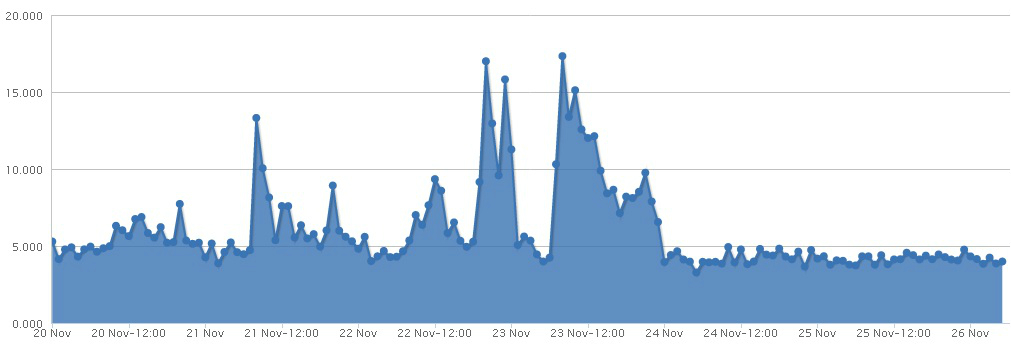
\includegraphics[scale=0.45]{grafico-black-friday.jpg}
	\caption{Tempo de resposta do \textit{Black Friday} Brasil 2012}
	\label{fig:grafico-black-friday}
	\fadaptada{blackfridayNews}
\end{figure}

As técnicas de gerenciamento de recursos são inúmeras, como as de inteligência artificial que utilizam lógica \textit{fuzzy}, algoritmos de mineração de dados e aprendizado de máquina \cite{Nobile2013}. As técnicas de aprendizado de máquina mostram-se interessantes para soluções imediatas, onde não há tempo hábil, inclusive, com abordagens não lineares empregadas para implementar um gerenciador de recursos responsável pela alteração dinâmica das capacidades computacionais. Outros trabalhos, como o \citeonline{Zhang2007}, buscam identificar padrões de comportamento na carga de trabalho e otimizar a provisão dinâmica de recursos nas máquinas virtuais com base em algoritmos reativos. \citeonline{Quiroz2009} buscam detectar, por monitoramento, a padronização e a tendência da carga de trabalho com o objetivo de otimizar os recursos. \citeonline{Nobile2013} também propõe o uso de modelos de séries temporais para modelagem de tráfego de tempo real e previsão de demanda, que é usada para criar partições de conexões para diferentes classes de prioridade.\citeonline{Zhang2011}, utiliza de técnicas de estatística e avaliação dos recursos disponíveis para tomar a decisão de qual recurso deve ser alocado.


\citeonline{Dong2014} afirmam que atualmente a maioria das aplicações Web são concebidas com sistemas \textit{mult-tiers} (multi-camadas) devido à flexibilidade de escalabilidade. O planejamento de capacidade é um passo importante para determinar a quantidade de recursos exigido para garantir determinada QoS. No entanto, em geral o planejamento de capacidade é basicamente uma decisão de longo prazo e quase estático, e os recursos são determinados pela taxa de utilização máxima da aplicação para evitar a pena excessiva de QoS.

\citeonline{Lourenco2015} afirmam que a partir de um planejamento de capacidade, a gestão de recursos em tempo real aumenta a sofisticação da arquitetura da solução nos diversos níveis e complexidade, as abordagens convencionais para análise de sistemas computacionais modernos; e concluí que as dinâmicas emergentes das interligações desses sistemas \textit{mult-tiers} pode produzir efeitos transitórios sobre o desempenho, como resposta temporal, ou o amortecimento e/ou comportamento oscilatório. Uma vez que estes efeitos variáveis no tempo podem potencialmente afetar a capacidade de resposta, eficiência e até mesmo a estabilidade global, métodos e ferramentas para avaliação das propriedades dinâmicas de sistemas computacionais são de importância prática para fins da engenharia.

Há caso em que existe o interesse em controlar a dinâmica deste sistema, para tanto é necessário modelar o sistema em questão e projetar um controlador que manipulará a sua dinâmica. Para trabalhar com estes sistemas deve-se ser capaz de modelar um sistema dinâmico, que em termos matemáticos é extrair um modelo matemático e analisar suas características dinâmicas. Um modelo matemático de um sistema dinâmico é definido como um conjunto de equações que representa a dinâmica de maneira relativamente razoável. Percebe-se que um modelo matemático não é exclusivo para um determinado sistema. Um sistema pode ser representando de muitas maneiras diferentes e, por conseguinte, podem ter diversos modelos matemáticos, dependendo da perspectiva, uns mais precisos que outros, e outros mais simplificados \cite{Ogata2001}.

Algumas vezes, é possível representar sistemas dinâmicos através de equações diferenciais obtidas com base nas leis básicas da física. Esses sistemas de equações diferenciais descrevem uma determinada dinâmica do sistema no domínio do tempo e, com o desenvolvimento dessas equações, é possível identificar propriedades fundamentais do sistema \cite{Nobile2013}. Quando a modelagem é muito dedutiva e muito complexa pode-se recorrer a métodos empíricos de identificação. Nesses, o modelo matemático é induzido mediante a comparação de entrada e saída.	


A avaliação por aferição, medição direta via instrumentação apropriada adequa-se nesse caso as necessidade; no entanto, é necessário a existência e disponibilidade do sistema ou protótipo, pois a avaliação é feita através de estímulos às entradas (\textit{benchmark}) e leitura de suas saídas, possibilitando testes de caixa preta em que não é exigido conhecimento sobre o funcionamento interno do sistema \cite{Nobile2013}, como em um sistema dinâmico, no qual o comportamento do sistema evolui com o tempo, em resposta a estímulos externos.

\section{Motivação}

Embora amplamente aplicada e difundida em diversas áreas da engenharia e ciência, a avaliação de desempenho em regime transitório é pouco explorada e usada em sistemas computacionais, em função de que sistemas computacionais e suas aplicações não tem necessita dessa analise. O desenvolvimento, contudo, de sistemas distribuídos de larga escala e complexidade altera essa realidade \cite{hpcs2015, Lourenco2015, medc}.

No \textit{\sigla{LaSDPC}{Laboratório de Sistemas Distribuídos e Programação Concorrente}}\footnote{\url{http://www.lasdpc.icmc.usp.br}}, onde desenvolve este projeto, trabalhos anteriores lidam com essa temática. O trabalho de \citeonline{Nobile2013}, um sistema com características dinâmicas, hospedado em um ambiente de computação em nuvem gerencia recursos elásticos por meio de mecanismos de provisão de QoS, técnicas de teoria de controle. Em outro trabalho, \citeonline{Lourenco2015} apresenta uma especificação de uma arquitetura conceitual que separa responsabilidades de simulação dinâmica em um conjunto de aspectos básicos, e formaliza um modelo de referência abstrata para a concepção de ferramentas de simulação. O trabalho de \citeonline{Edwin2015}, em desenvolvimento também no LaSDPC, estuda e define uma metodologia de análise transiente dedicado a sistemas computacionais dinâmicos reais utilizando da especificação arquitetural proposto por \citeonline{Lourenco2015}. A principal contribuição pretendida é a formulação e definição de uma metodologia para seu emprego em sistemas, cuja a metodologia deverá ser capaz de descrever e especificar os passos para modelar o sistema, e analisar os resultados transiente mediante as variações na carga de trabalho. Para tanto, o trabalho de \citeonline{Edwin2015} utiliza de um \textit{benchmark} para a validação experimental de sua metodologia. No entanto, o \textit{benchmark} escolhido por \citeonline{Edwin2015}, Bench4Q, não contempla das especificações apresentadas por \citeonline{Lourenco2015}.

Segundo \citeonline{Binnig2009} os \textit{benchmarks} tradicionais não são suficientes para a análise desses novos serviços de elasticidade da computação em nuvem. O principal desafio dos novos \textit{benchmarks} é fazer com que as métricas ofereçam informações relevantes a esses diferentes serviços e com diferentes capacidades e garantias desses serviços. \citeonline{Dong2014} afirmam que, a maioria das aplicações Web são concebidas como sistemas \textit{mult-tiers}, devido à flexibilidade e capacidade de reutilização de \textit{software}, porem é difícil de modelar o comportamento de aplicações Web de \textit{multi-tiers}, devido ao fato de que a carga de trabalho estimula a dinâmica do sistema nos diferentes níveis da camada.

No âmbito da análise de desempenho em sistemas computacionais, definimos o \textit{benchmarking} como o ato de medir e avaliar o desempenho computacional, protocolos de rede, dispositivos e redes, sob condições de referência, em relação a uma avaliação de referência. O objetivo deste processo de \textit{benchmarking} é permitir a comparação equitativa por diferentes soluções, ou entre desenvolvimentos subsequentes de um \textit{\sigla{SUT}{\textit{System Under Test}}}. \textit{Benchmarking} é o principal método para medir o desempenho de uma máquina ou sistema.

Apesar de existam diversos \textit{benchmarks} e ferramentas para o estudo, nenhuma delas estimulam a dinâmica transiente do sistema e permite uma avaliação em regime transiente, que se faz necessário para a pesquisa de \citeonline{Edwin2015}. A proposta deste trabalho é identificar um \textit{benchmark} e adequá-lo de maneira em que estimule a dinâmica do sistema possibilitando uma avaliação transiente.


\section{Objetivo}
Este trabalho tem por objetivo a extensão do \textit{framework} de \textit{benchmark} Bench4Q afim de atender os requisitos do modelo \textit{\sigla{MEDC}{\textit{Monitor, Effector, Demanda and Capacity}}}, proposto por \citeonline{Lourenco2015}. O objetivo restringe-se ao módulo de modulação da carga de trabalho, gerado pelo \textit{benchmark}, acrescendo-o de provisões nativas para gerar perturbações capazes de excitar e produzir o regime transiente do sistema SUT do \textit{benchmark}, permitindo apreciar-se sua dinâmica. A contribuição almejada é a disponibilização de um \textit{benchmark} que auxilie a análise de sistemas dinâmico e que possibilite a analise transiente.

